\section{\dataset}
% \subsection{Obtaining Realistic and Diverse Human-Aligned Activity Definitions}
\label{sec:activity}
% Once activity topics have been sourced to be distributed by human need, they need to be defined concretely. These definitions should reflect intuitive, human instantiations of the activity topics.

\begin{figure}[t]
    \centering
    % IMPORTANT! IF YOU NEED TO MAKE THIS FIGURE SMALLER, ASK CEM TO MAKE HIGHER ASPECT RATIO VERSION SO THAT IT STILL LOOKS FULL-WIDTH
    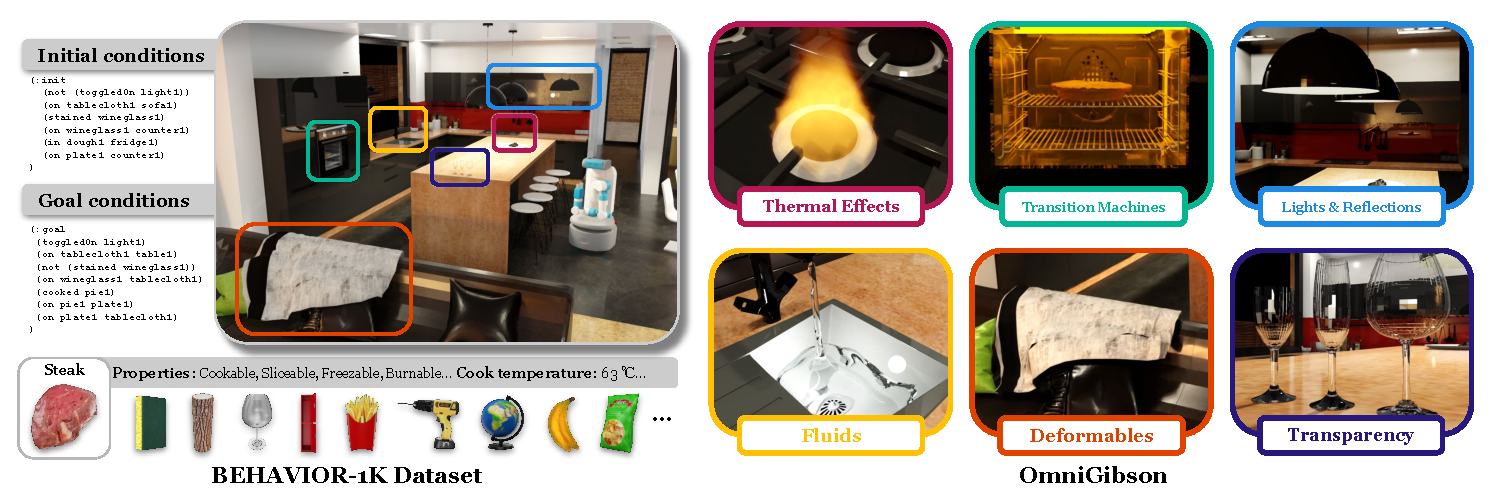
\includegraphics[width=\textwidth]{figures/models/scene_features.pdf}
    \caption{\textbf{Elements of \benchmark.} Our benchmark comprises two elements: \dataset and \simulator. Left: \dataset includes 1,000 BDDL activity definitions (top left), 50 realistic and diverse scenes (top right), and 9,000+ objects with properties annotated in the knowledge base (bottom). Right: \simulator provides the necessary functionalities to realistically simulate the 1000 activities, including thermal effects such as fire/steam/smoke (top left), fluid dynamics (bottom left), functional machines for transition rules (top center), deformable bodies/cloths (bottom center), realistic lighting and reflections (top right), and transparency rendering (bottom right). Together, they constitute a concrete, realistic instantiation of an everyday activity like \texttt{CookingDinner} in simulation.}%A \benchmark scene such as the house scene shown here contains many articulated objects to support this rich set of features.}
    \label{fig:model_vis}
\end{figure}

Once activities have been sourced to reflect human needs, they need to be concretely defined and instantiated the way they would occur in the real world. We build the \dataset, which includes a knowledge base of crowdsourced activity definitions with relevant objects and object states, and a large-scale repository of high-quality, interactive 3D models.

% Sanjana, an important change: we are merging 4.1 and 4.2 and reduce 4.2 to one paragraph. The beginning of 4.1 now will be the beginning of 4. Let me give you some glue starting point - ok
% or you can give it a try. just mention that we creating a database that includes activity defs, knowledge base and models 
% - gave it a pass 

%To get activity definitions that represent human need yet can be simulated and interpreted as reward,
We crowdsource concrete definitions of activities in the form of \bddlfull (\bddl)~\cite{srivastava2021behavior}. \bddl is based on predicate logic and designed to be accessible for laypeople to describe concrete initial and goal conditions for a given activity. Unlike geometric, image/video, or experience goal specifications~\cite{batra2020rearrangement, weihs2021visual}, \bddl definitions are in terms of objects and object states, allowing annotators to define at an intuitive semantic level. The semantic symbols also capture the fact that multiple physical states might be valid initializations and solutions to an activity. See Listings~\ref{lst:bddl3},~\ref{lst:bddl4} and~\ref{lst:bddl5} in Appendix for example definitions.

% To get such representative definitions, \benchmark activities are defined by lay annotators. Crowdsourcing 1,000 ecologically plausible task definitions that can be simulated and interpreted as reward requires a systematic, accessible process. \benchmark definitions are therefore written in \bddlfull (\bddl)~\cite{srivastava2021behavior}. \bddl is based in predicate logic and has custom operators designed for usability, making it a natural way to express concrete initial scenes and general desired goals. Its terms and predicates are objects and states the objects can be in; the annotators are therefore able to write definitions at a semantic level that is more intuitive than arbitrary geometry. The semantic symbols also capture the fact that multiple physical states may be valid initializations and solutions to a task.

The object and object state spaces that activity definitions are built upon are annotated to be ecologically plausible. The object spaces are derived from 5,000 WikiHow articles for the 1,000 activities and mapped to 2,964 leaf-level synsets either from WordNet~\cite{wordnet} or custom-designed. Through crowdworkers, students, and GPT-3~\cite{gpt3}, we also associate each object with our fully simulatable object states: for example, \texttt{apple} is associated with \texttt{cooked} and \texttt{sliced}, but not \texttt{toggledOn}.
%These associations are activity-agnostic, since simulating irrelevant and undesirable states provides important learning signals. 
Many object-property pairs are augmented with parameters, e.g., ``cooked temperature for apples'', taking advantage of \simulator's continuous extended states to make activities especially realistic. Finally, annotators and researchers also create transition rules, e.g., turning tomatoes and salt into sauces, or requiring sandpaper to remove rust. The result is a knowledge base of tens of thousands of elements underlying 1000 ecologically plausible activity definitions. We ensure annotation quality by having five experienced machine learning annotators verify a subset of all types of annotations and receive extremely high approval rates ($>$96.8\%). See Appendix~\ref{as:act_ann} for more details about the knowledge base.

% Along with \bddl to provide intuitive structure, annotators are given ecologically plausible spaces of objects and object states to build definition content from. As seen in Fig.~\ref{fig:activity_pipeline}, we recruit \todo{X} crowdworkers and \todo{Y} students to collect 4,500 WikiHow articles from which we extracted \todo{X} noun phrases and mapped them to 1,484 WordNet~\cite{wordnet} synsets that form \benchmark's object space. With crowdworkers, students, and GPT-3~\cite{gpt3} we also collect annotations for each object with nine unary object states (e.g. ``cooked'', ``toggled on''), four binary states (e.g. ``filled'', ``on top''), and one variable-arity state (``mixed''). Over 20 more states are inferred from these annotations. For eight states and every object they applied to, students also collect parameters (e.g. object-specific ``cook temperature''s). Annotators and researchers finally create realistic cleaning and cooking transitions (such as turning tomatoes and salt into sauce, or using specifically sandpaper to deal with rust instead of a generic cleaning solution) for over 150 activities. 

% We ensure annotation quality by having five experienced machine learning annotators verify 10\% of every crowdsourced or GPT-3-generated pipeline step. All object- and object state-related annotations have >96.8\% approval, and activity definitions have >4.85/5.0 Likert scores for all approval survey questions (see Appendix for details). Furthermore, the goals are verified as logically solvable with \bddl's solver, and the custom annotation software guarantees simulatability in \simulator.

% These rich annotations result in 900 \bddl definitions (examples in fig.~\ref{fig:activity_definition_examples}). To ensure the quality of annotations, we conduct quality assessment by randomly samping 10\% of each annotation generated via crowdsourcing or a learned method, and send them to five experienced machine learning data annotators to verify. The average approval rate is \todo{X} (see Appendix for details).

% Along with \bddl to provide intuitive structure, annotators are given ecologically plausible spaces of objects and object states to build definition content from. Fig.~\ref{fig:activity_pipeline} outlines each step of this data collection: overall, we collect 4,500 WikiHow articles, extract \todo{XX} noun phrases from them, and finalize 1,484 object terms that span the object spaces of each activity. Each object term is mapped to a WordNet~\ref{wordnet} synset, eliminating ambiguity and providing taxonomic structure. We associate each of these objects with over 35 fully simulated object states, thereby collecting over 50,000 annotations from humans and GPT-3~\cite{gpt3}

% Activity definition results (referring to Table 1)
% With this pipeline, we recruited X humans (X upworkers, Y students) work on ...
% 4500 articles, X noun phrases, X objects, X object states (X unary Y binary Z unary, can use a few examples), X types of transition maps (including recipes),  X object state parameters, which lead to 900 BDDL definitions. Example BDDL definitions can be seen in Fig.~\ref{fig:activity_definition_examples}. To ensure the quality of annotations, we conduct quality assessment by randomly sample x\% of annotations, and send them to X to verify. The average approval rate is X (see Appendix for details). 

The diversity of these activity definitions requires diverse object and scene models. % and (b) realistic simulation of different physical states and processes (see Sec.~\ref{sec:simulation}). 
On top of the 15 house scenes from \oldbenchmark~\cite{srivastava2021behavior}, we acquire 35 fully interactive scenes across diverse scene types, such as gardens, offices, restaurants, and stores, that are essential for everyday activities. This is unprecedented compared to other benchmarks (see Table~\ref{tab:comparingbenchmarks}). We also acquire 9,000+ object instances across 1,900+ categories required by the activities, and annotate rich physical (e.g., friction, mass, articulation) and semantic properties (e.g., category) for each object. Representative scene and object models can be seen in Fig.~\ref{fig:model_vis}. More details of the 3D models can be found in Appendix~\ref{as:modeling}.

% bddl1: simple, involves substances and complex cleaning 
% bddl2: moderate, involves assembly? 
% bddl3: most complex, involves comp/decomp
% bddl4: b100 - some pick and place that involves basic cleaning 
% bddl5: b100 - some long pick and place
% \todo{cite gpt3}



% \item All previous common sense knowledgebase are insufficient due to B1K's diversity (Table \ref{tab:activity_cskb}), so we create B1K dataset to support B1K activity definition. 

% - good benchmarking and simulation requires parametrization with data that is 
%     - ecologically plausible 
%     - grounded in human preference
% - Prior work?
%       - at least involve it so i can cite all the other benchmarks 
% - Definitions - two parts, the underlying data and the symbolic language for specification
% - Annotations to get data for definitions
%     - Realistic 
%     - Grounded 
%     - Human preference
% - Symbolic language
%     - Human preference: semantic, custom quantifiers 
%     - Eco plaus: all kinds of new features
%           - cite prior attempts 
%     - BDDL repo
% - Definition annotations
%     - Interface
% - Quality metrics
% - BEHAVIOR symbolics create appropriate challenge
% - Impact



% Once activity topics have been sourced to be distributed by human need, they need to be defined concretely. These definitions should reflect intuitive, human instantiations of the activity topics, and have the richness seen for the same task in the real world. 

% To get such representative definitions, \benchmark activities are defined by lay annotators. Collecting ecologically plausible task definitions that can be simulated is a major design problem. Collecting 1,000 requires a systematic process, and crowdsourcing requires it to be accessible. We therefore use \bddlfull (\bddl)~\cite{srivastava2021behavior} and offer annotators a visual versoin~\cite{srivastava2021behavior}. \bddl is predicate logic-based and inspired by PDDL~\cite{mcdermott1998pddl}, with custom operators to make it more accessible. As a formalization of human reasoning, it is a natural way to describe an environment and express desired goals. In \bddl, logic constants and variables are objects and predicates are states of the objects, meaning the definitions are built at a semantic level. The semantic symbols are intuitive for laypeople, and they capture the fact that there are multiple reasonable simulator configurations that both instantiate and solve these complex and naturalistic tasks.
% \todo{correctly reference supplementary bddl}

% To ensure that not only the structure but the content of the definitions are as reflective of human need as possible, we equip annotators with ecologically plausible object spaces and realistic object-state associations. Each activity's object space is sourced from from five relevant WikiHow~\cite{wikihow} articles, since WikiHow is a prevalent and crowdsourced database of items needed to do a task. Each object is mapped to a WordNet~\cite{wordnet} synset to avoid word sense ambiguity and obtain taxonomic structure in the object space. These objects are then associated with each of our 35+ fully simulated object states\textemdash for example, ``apple'' is associated with ``cooked'' and ``frozen'' but not ``toggled on''. Associations are determined activity-agnostically because it should always be possible to enter irrelevant and undesired object states, as common sense and safety signals are important to learning human need. Object-state associations are also annotations, collected from foundation models (FMs)~\cite{bommasani2021opportunities}, specifically GPT-3~\cite{gpt3}, or humans where necessary. This set of sources makes the definition substrates ecologically plausible and scalable to collect. 

% The combination of intuitive, semantic \bddl structure and ecologically plausible content spaces make it possible for us to collect naturalistic definitions that are free from researcher bias at scale. Lsts.~\ref{lst:bddl1},~\ref{lst:bddl2}, and~\ref{lst:bddl3} show \benchmark definitions of increasing difficulty. Compared to \bddl definitions from \oldbenchmark (lsts.~\ref{lst:bddl4} and~\ref{lst:bddl5}, the activity length is of similar range but the expressiveness is much higher - in \benchmark, arbitrarily subdividable substances like flour or juice can be represented generally as objects and cleaning is more substance-specific than simply cleaning implement and water, and we can transform sets of objects into new objects as in building or cooking.








